\documentclass{article}

% Symbols
\usepackage{amsfonts, amsthm}
\usepackage{upgreek}
\usepackage{physics}
\usepackage{cancel}
\usepackage{amssymb, latexsym, amsmath}

%Algorithms
\usepackage[ruled,lined,linesnumbered,commentsnumbered]{algorithm2e}

%% Identación
\setlength{\parindent}{0cm}

% Código
\newcommand{\code}[1]{\textcolor{white!25!black}{\texttt{#1}}}
\usepackage{listings}

%AMS
\usepackage{amsthm}
\newtheorem{algo-thm}{Algoritmo}

% Graphics
\usepackage{graphicx}
\usepackage{pgf}

% Margins
\addtolength{\voffset}{-1.5cm}
\addtolength{\hoffset}{-1.5cm}
\addtolength{\textwidth}{3cm}
\addtolength{\textheight}{3cm}

%Header-Footer
\usepackage{fancyhdr}
\renewcommand{\headrulewidth}{1pt}

\newcommand{\set}[1]{
  \left\{ #1 \right\}
}

\footskip = 50pt
\renewcommand{\headrulewidth}{1pt}

\pagestyle{fancyplain}

\begin{document}
\title{UNIVERSIDAD NACIONAL AUT\'ONOMA DE M\'EXICO\\ Facultad de Ciencias}
\author{Integrantes:\\
  Marco Silva Huerta\\
  Adri\'an Aguilera Moreno\\}
\date{}
\maketitle
\begin{center}
  
\includegraphics[scale=0.20]{../Imagen/Portada.jpg}\\[0.4cm]
  \Large
  \bf{Lógica Computacional}
  \normalsize
\end{center}
\newpage
\fancyhead[r]{ Lógica Computacional 2022-2}
%%%%%%%%%%%%%%%%%%%%%%%%%%%%%%%%%%%%%%%%%%%%%%%%%%%%%
\section*{\LARGE{Práctica 5}}
%%%%%%%%%%%%%%%%%%%%%%%%%%%%%%%%%%%%%%%%%%%%%%%%%%%%%%%%%%%%%%%%%%%%%
%%%%%%%%%%%%%%%%%%%%%%% ESPECIFICACIONES AQUÍ %%%%%%%%%%%%%%%%%%%%%%%
%%%%%%%%%%%%%%%%%%%%%%%%%%%%%%%%%%%%%%%%%%%%%%%%%%%%%%%%%%%%%%%%%%%%%
\newcommand{\localtextbulletone}{\textcolor{black}{\raisebox{.45ex}{\rule{.6ex}{.6ex}}}}
\renewcommand{\labelitemi}{\localtextbulletone}
\begin{itemize}
\item Ejercicio 2.

  \code{trayectoria\_ida}: este predicado usa la idea que vimos en clase
  con la profesora (la idea con gráficas). Así, tenemos una adyacencia
  entre estaciones, y queremos saber si existen trayectorías (el definir
  las adyacencias es trivial), luego tomamos dos estaciones a definir si
  existen trayectorías entre estas. Para saber lo anterior basta tomar
  un caso recursivo (en el caso, en que no son adyacentes las estacuiones),
  si la estación A tiene de por medio alguna estación B para llegar a C
  entonces se toma la adyacenccia de AB y se llama nuevamente al predicado
  \code{trayectoria\_ida} con parámetros BC. Esto funciona para cualesquiera
  estaciones en las que haya trayectoria, pero solo  en una dirección (pues
  por alguna razón el regreso entra en un bucle recursivo).
  
  \code{camino}: este predicado nos regresa una lista (que debemos pasar
  por parámetro para que el algoritmo la llene) con las estaciones a
  recorrer de entre dos partículares A y B, incluyendose. Aquí, nos pareció
  mejor mandar a llamar al predicado del inciso (c) que al del inciso (a),
  pues es más completo al recorrer en ambos sentidos las estaciones.
  
  \code{es\_camino}: es una mejor implementación del inciso (a), pues
  nos pareció mejor idea mejorar (a), que implementarlo invertido.
  
  \textbf{Ejemplo de prueba:}
  \begin{center}
    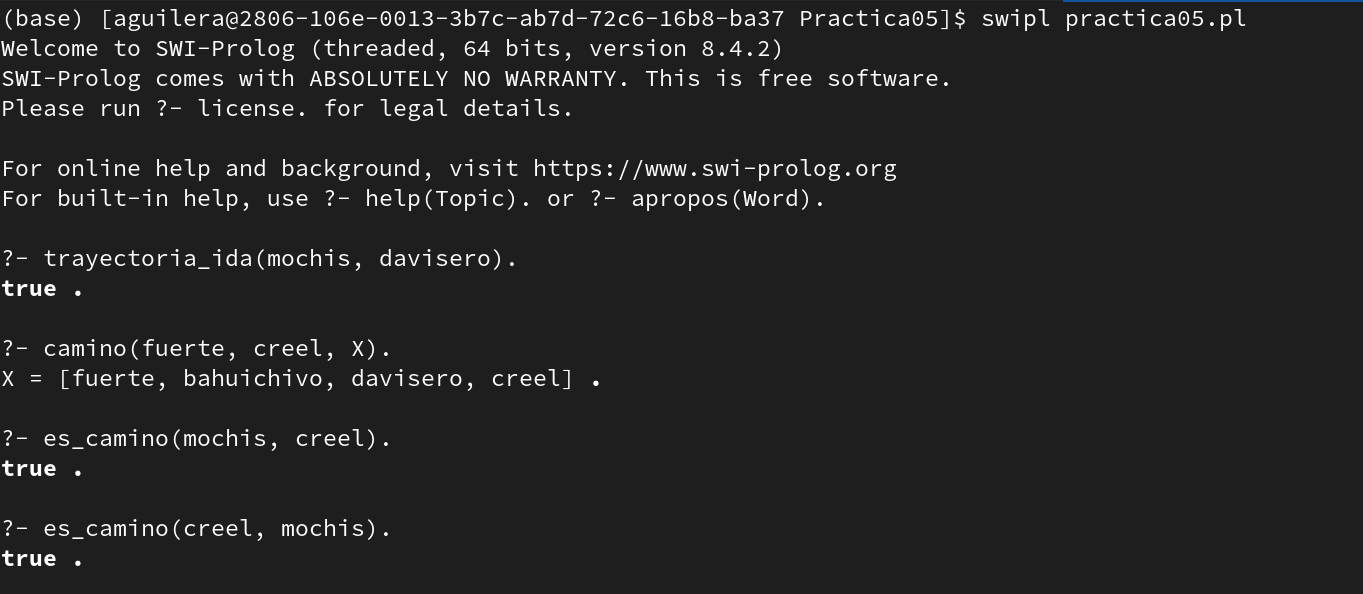
\includegraphics[scale=0.30]{./CasoPruebaEjercicio2.png}\\[0.4cm]
  \end{center}
\item Ejercicio 4. Para este caso se analizan dos posibles casos,
  cuando la lista es vacía y cuando tiene elementos.
\item Ejercicio 5.
  Aquí se analizan diversos predicados, que por considerarlos triviales
  solo anexamos un ejemplo de ejecución.
  
  \textbf{Ejemplo de prueba:}
  \begin{center}
    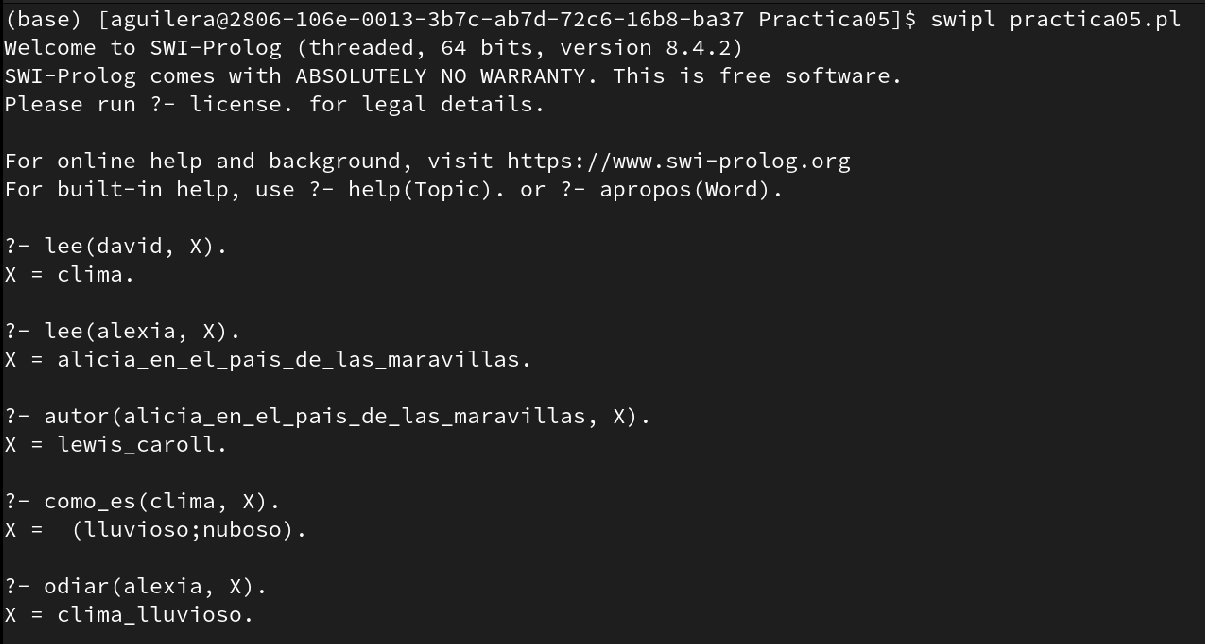
\includegraphics[scale=0.30]{./CasoPruebaEjercicio5.png}\\[0.4cm]
  \end{center}
  
\item Ejercicio 6. Para el predicado \code{abuelo} se realizó un análisis
  del párrafo, entonces se declaran 5 posibles hechos (con el nombre del
  predicado \code{esta\_relacionado}) con base a esta información y por
  medio del caso depediente del predicado mencionado con anterioridad se
  da la relación buscada.
\end{itemize}
\begin{center}
  \fbox{
    \begin{minipage}[b][1\height]%
      [t]{0.867\textwidth}
      Matriculas:
      \begin{itemize}
      \item[1.] Marco Silva Huerta: 316205326.
      \item[2.] Adrian Aguilera Moreno: 421005200.
      \end{itemize}
  \end{minipage}}
\end{center}

\end{document}
